\documentclass[authoryear,5p]{elsarticle}

\renewcommand{\today}{}  % Get rid of date on footer
\journal{Ann. Nucl. Energy}

\usepackage[bitstream-charter]{mathdesign} % Use BT Charter font
\usepackage[T1]{fontenc}                   % Use T1 encoding instead of OT1
\usepackage[utf8]{inputenc}                % Use UTF8 input encoding
\usepackage{microtype}                     % Improve typography
\usepackage{amsmath, mathtools}             % AMS Math extensions
\usepackage{booktabs}                      % Improved table spacing
\usepackage{booktabs}
\usepackage{siunitx}
\usepackage{breqn}
\usepackage{nicefrac}

\usepackage[breaklinks=true]{hyperref}

\usepackage{subcaption}
\usepackage{dblfloatfix}
\usepackage{color}

%\usepackage{algorithmic,eqparbox,array}
%\renewcommand\algorithmiccomment[1]{
%  \hspace{\fill}\#\ \eqparbox{COMMENT}{#1}
%}

\usepackage{todonotes}

\usepackage[labelfont=bf]{caption}
\captionsetup[figure]{labelsep=period, name=Figure}
\captionsetup[table]{labelsep=period, name=Table}
\def \figureautorefname {Figure}
\def \algorithmautorefname {Algorithm}

\usepackage[scaled]{beramono}

\usepackage{etoolbox}
\usepackage{listings}
\usepackage{color}

% Algorithm constructs
\usepackage{algorithm} % Provides algorithm environment
\usepackage{algorithmicx}       % Provides algorithmic block
\usepackage{algpseudocode}      % Option of algorithmicx package
\renewcommand{\thealgorithm}{\thechapter-\arabic{algorithm}}
\newcommand\Algphase[1]{%
\vspace*{-.7\baselineskip}\Statex\hspace*{\dimexpr-\algorithmicindent-2pt\relax}\rule{\columnwidth}{0.4pt}%
\Statex\hspace*{-\algorithmicindent}{#1}%
\vspace*{-.7\baselineskip}\Statex\hspace*{\dimexpr-\algorithmicindent-2pt\relax}\rule{\columnwidth}{0.4pt}%
}
\newcommand{\algrule}[1][.4pt]{\par\vskip.5\baselineskip\hrule height #1\par\vskip.5\baselineskip}

\lstset{
  language=Python,
  showstringspaces=false,
  formfeed=\newpage,
  tabsize=4,
  commentstyle=\itshape,
  basicstyle=\ttfamily,
  morekeywords={models, lambda, forms},
  frame=single
}

\newcommand{\code}[2]{
  \subsection*{#1}
  \lstinputlisting{#2}
}

\def\sectionautorefname{Sec.}
\def\subsectionautorefname{Sec.}
\def\equationautorefname{Eq.}
\def\figureautorefname{Fig.}
\def\algorithmautorefname{Alg.}

\hypersetup{colorlinks=true,
  pdftitle={An Analysis of Condensation Errors in Multi-Group Cross-Section Generation for Fine-Mesh Neutron Transport Calculations},
  pdfauthor={William Boyd, Nathan Gibson, Benoit Forget and Kord Smith.}}

\begin{document}

\begin{frontmatter}

\title{An Analysis of Condensation Errors in Multi-Group Cross-Section Generation for Fine-Mesh Neutron Transport Calculations}

\author{William Boyd\corref{cor1}}
\ead{wboyd@mit.edu}

\author{Nathan Gibson\corref{}}
\ead{nathan.gibson@unnpp.gov}

\author{Benoit Forget\corref{}}
\ead{bforget@mit.edu}

\author{Kord Smith\corref{}}
\ead{kord@mit.edu}

\address{Massachusetts Institute of Technology, Department of Nuclear Science and Engineering, 77 Massachusetts Avenue, Building 24, Cambridge, MA 02139, United States\vspace{-8ex}}


%%%%%%%%%%%%%%%%%%%%%%%%%%%%%%%%%%%%%%%%%%%%%%%%%%%%%%%%%%%%%%%%%%%%%%%%%%%%%%%
\begin{abstract}
%%%%%%%%%%%%%%%%%%%%%%%%%%%%%%%%%%%%%%%%%%%%%%%%%%%%%%%%%%%%%%%%%%%%%%%%%%%%%%%

\end{abstract}

\begin{keyword}
Multi-group cross-sections, energy condensation, spatial homogenization, superhomog\'{e}n\'{e}isation factors
\end{keyword}

\end{frontmatter}

%
%%%%%%%%%%%%%%%%%%%%%%%%%%%%%%%%%%%%%%%%%%%%%%%%%%%%%%%%%%%%%%%%%%%%%%%%%%%%%%%%
%\section*{Ben's Outline}
%%%%%%%%%%%%%%%%%%%%%%%%%%%%%%%%%%%%%%%%%%%%%%%%%%%%%%%%%%%%%%%%%%%%%%%%%%%%%%%%

%\begin{itemize}
%\item Problem Statement
%\begin{itemize}
%\item Cross section collapse cannot preserve reaction rates
%\item SPH factors, heterogeneity factors, discontinuity factors
%\end{itemize}
%\item 1D analysis (or 2D Fake)
%\begin{itemize}
%\item Methodology for you 1D slab with single square/SLBW resonance (MOC/CPM solver)
%\item Tables of error by
%\begin{itemize}
%\item resonance peak
%\item resonance width
%\item group width
%\end{itemize}
%\item Angular dependent xs coupled with spatial discretization
%\end{itemize}
%\item 2D analysis (or 2D Real)
%\begin{itemize}
%\item Continuous energy, multi-nuclide, 4 region pin cell
%\item show bias for 2-70 groups (CASMO structures)
%\begin{itemize}
%\item Full OpenMC
%\item Iso-in-lab
%\item Spatial discretization
%\item show effect of discretizing resonance
%\end{itemize}
%\item look at groupwise flux and pcm errors by region, isotope
%\item fixed source OpenMC-OpenMOC shows same phenomenon
%\item SPH factors from OpenMOC by group/region
%\end{itemize}
%\item Possible solutions
%\begin{itemize}
%\item Angular dependent XS
%\item SPH vs just fudging transport xs
%\item Absorption rate in U238 vs SPH factor by resonance group
%\end{itemize}
%\end{itemize}

%%%%%%%%%%%%%%%%%%%%%%%%%%%%%%%%%%%%%%%%%%%%%%%%%%%%%%%%%%%%%%%%%%%%%%%%%%%%%%%
\section{Introduction}
\label{sec:intro}
%%%%%%%%%%%%%%%%%%%%%%%%%%%%%%%%%%%%%%%%%%%%%%%%%%%%%%%%%%%%%%%%%%%%%%%%%%%%%%%

The nuclear reactor physics community has long strived for deterministic neutron transport-based tools for whole-core reactor analysis. A key challenge for whole-core multi-group transport methods is accurate reactor agnostic multi-group cross section (MGXS) generation. The MGXS generation process applies a series of approximations to produce spatially homogenized and energy condensed MGXS in each spatial zone and energy group. Many approximations related to multi-group theory, including the selection of discretized energy group structures and the truncation of the Legendre expansion of the multi-group scattering kernel, are widely studied in the literature. However, the practical impact of the flux separability approximation, which permits the use of the scalar rather than the angular neutron flux to weight the continuous energy cross sections, is less understood. This paper investigates the flux separability approximation and quantifies its significance for heterogeneous PWR problems.

This work employs Monte Carlo (MC) neutron transport simulations to generate MGXS. Monte Carlo methods have increasingly been used to generate few group constants for coarse mesh diffusion, most notably by the Serpent MC code \citep{serpent2013manual}, and to a much lesser extent, for high-fidelity neutron transport methods \citep{redmond1997multigroup, nelson2014improved, cai2014condensation, boyd2016thesis}. The advantage of a MC-based approach is that all of the relevant physics are directly embedded into MGXS by weighting the continuous energy cross sections with a statistical proxy to the ``true'' neutron flux. However, this paper shows that even when the ``true'' scalar flux is used to generate MGXS, the flux separability approximation results in a non-negligible eigenvalue bias between continuous energy and multi-group calculations due to under-prediction of U-238 capture in resonance energy groups.

% In addition, a reference solution may be directly computed from the same MC simulation to compare with the multi-group transport solution.

The content in this paper is organized as follows. The flux separability approximation is introduced in~\autoref{sec:flux-separability}. The methodology used to rigorously quantify the impact of the approximation on PWR problems -- including two benchmark problems and simulation tools -- are described in~\autoref{sec:methodology}. \autoref{sec:test-case1} presents a toy problem which illustrates how scalar flux-weighting of the cross sections cannot preserve the reaction rate for a single resonant energy group, while \autoref{sec:test-case2} investigates the flux separability approximation in the context of a fully-detailed, critical PWR fuel pin cell. SuPerHomog\'{e}n\'{e}isation (SPH) factors is explored in~\autoref{sec:sph} as one possible solution to this approximation, while other approaches, including angular-dependent MGXS, are outlined in~\autoref{sec:conclusions}.
%%%%%%%%%%%%%%%%%%%%%%%%%%%%%%%%%%%%%%%%%%%%%%%%%%%%%%%%%%%%%%%%%%%%%%%%%%%%%%%
\section{Flux Separability Approximation}
\label{sec:flux-separability}
%%%%%%%%%%%%%%%%%%%%%%%%%%%%%%%%%%%%%%%%%%%%%%%%%%%%%%%%%%%%%%%%%%%%%%%%%%%%%%%

The multi-group approach used to solve the transport equation subdivides the neutron's energy into discrete bins known as energy groups. The energy groups are indexed starting at 1 for high energies and ending with $G$ for the lowest energies of interest. The MGXS are the averages of the corresponding continuous energy cross sections weighted by the angular neutron flux $\psi$ in each energy group:

\begin{dmath}
\label{eqn:sigt-mg}
\Sigma_{t,g}(\mathbf{r},\mathbf{\Omega}) \equiv \frac{\int\displaylimits_{E_{g}}^{E_{g-1}} \Sigma_{t}(\mathbf{r},E)\psi(\mathbf{r},\mathbf{\Omega},E)\mathrm{d}E}{\psi_{g}(\mathbf{r},\mathbf{\Omega})}
\end{dmath}

The angular dependence of the total cross section is often treated with the flux separability approximation. Flux separability makes the simplifying assumption that the energy and angular dependence of the flux varies independently such that the angular flux can be written as the product of the scalar neutron flux $\phi(\mathbf{r},E)$ and some function $W(\mathbf{r}, \mathbf{\Omega})$:

\begin{dmath}
\label{eqn:flux-separate}
\psi(\mathbf{r},\mathbf{\Omega},E) = \phi(\mathbf{r},E) W(\mathbf{r},\mathbf{\Omega})
\end{dmath}

\noindent The angular dependence of the $\Sigma_{t,g}$ may then be eliminated by inserting Eqn.~\ref{eqn:flux-separate} into Eqn.~\ref{eqn:sigt-mg}, factoring out $W(\mathbf{r},\mathbf{\Omega})$ and writing $\Sigma_{t}$ in terms of the scalar flux:

\begin{dmath}
\label{eqn:sigt-mg-scalar}
\Sigma_{t,g}(\mathbf{r}) \equiv \frac{\int\displaylimits_{E_{g}}^{E_{g-1}} \Sigma_{t}(\mathbf{r},E)\phi(\mathbf{r},E)W(\mathbf{r},\mathbf{\Omega})\mathrm{d}E}{\phi_{g}(\mathbf{r})W(\mathbf{r},\mathbf{\Omega})} = \frac{\int\displaylimits_{E_{g}}^{E_{g-1}} \Sigma_{t}(\mathbf{r},E)\phi(\mathbf{r},E)\mathrm{d}E}{\phi_{g}(\mathbf{r})}
\end{dmath}

Although flux separability is a simple and commonly used approach to reduce the complexity of the ``true'' multi-group total cross section, it is not always valid and may not preserve neutron balance.

%%%%%%%%%%%%%%%%%%%%%%%%%%%%%%%%%%%%%%%%%%%%%%%%%%%%%%%%%%%%%%%%%%%%%%%%%%%%%%%
\section{Methodology}
\label{sec:methodology}
%%%%%%%%%%%%%%%%%%%%%%%%%%%%%%%%%%%%%%%%%%%%%%%%%%%%%%%%%%%%%%%%%%%%%%%%%%%%%%%

Two case studies were used to disaggregate the approximation errors inherent to deterministic multi-group transport methods from the component error specific to the flux separability approximation. Ultra-fine deterministic and continuous energy Monte Carlo transport methods were used to collapse multi-group cross sections and generate reference solutions for each case study as discussed in~\autoref{subsec:test-case1} and~\autoref{subsec:test-case2}, respectively. Both case studies modeled a multi-region PWR fuel pin geometry with varying levels of complexity. The two analyses isolate the impact of the flux separability approximation on local reaction rates, as well as demonstrate the compounding effect of errors in each energy group on the $k$-eigenvalue. The following sections discuss the benchmark specifications and simulation tools used by each case study.

% hammer home that all of this is due to heterogeneous effects:


%%%%%%%%%%%%%%%%%%%%%%%%%%%%%%%%%%%%%%%%%%%%%%%%%%%%%%%%%%%%%%%%%%%%%%%%%%%%%%%
\subsection{Test Case 1: Resonance with Slowing Down Source}
\label{subsec:test-case1}

%%%%%%%%%%%%%%%%%%%%%%%%%%%%%%%%%%%%%%%%%%%%%%%%%%%%%%%%%%%%%%%%%%%%%%%%%%%%%%%
\subsubsection{Benchmark Problem}
\label{subsubsec:benchmark-case1}

The first test case modeled a simple benchmark problem in which the reference flux could be computed precisely to demonstrate the existence of errors from approximately collapsing Eqn.~\ref{eqn:transport-eqn-ce} into Eqn.~\ref{eqn:transport-eqn-mg-separate} with the flux separability approximation. The first test case problem consisted of a unit cell of an infinite array of unclad fuel pins. The fuel material contained U-238 with an atom density of 0.022 $\nicefrac{\text{a}}{\text{b-cm}}$ and a purely scattering nuclide with a constant cross section of 0.176 cm\textsuperscript{-1}, an analog to oxygen in UO\textsubscript{2}. The moderator was a pure scatterer with a constant cross section of 1.23 cm\textsuperscript{-1}. The pin radius is 0.4 cm and the pitch was 1.26 cm. The source was given by the scatter source from the narrow resonance approximation:

\begin{dmath}
\label{eqn:test-source-ce}
Q(\mathbf{r},\mathbf{\Omega},E) = \frac{1}{4\pi} \frac{\Sigma_{p}(\mathbf{r})}{E}
\end{dmath}

% do you (instead) have a case where you analyze a single resonance with different peak/widths???

%%%%%%%%%%%%%%%%%%%%%%%%%%%%%%%%%%%%%%%%%%%%%%%%%%%%%%%%%%%%%%%%%%%%%%%%%%%%%%%
\subsubsection{Simulation Tools}
\label{subsubsec:sim-tools-case1}

A reference continuous energy flux was computed for the first test case by solving Eqn.~\ref{eqn:transport-eqn-mg-separate} for each energy point {\color{red}[using a toy MOC code? Spatial and angular discretization?]}. The reference reaction rates in each region were obtained by integrating the flux multiplied by a cross section over an energy range of interest and over the volume of the fuel pin. The total cross section was collapsed using the reference flux according to Eqn.~\ref{eqn:sigt-mg-scalar}, and the source was collapsed as follows:

\begin{dmath}
\label{eqn:test1-source-mg}
Q_{g}(\mathbf{r},\mathbf{\Omega}) = \int\displaylimits_{E_{g}}^{E_{g-1}} Q(\mathbf{r},\mathbf{\Omega},E)\mathrm{d}E
\end{dmath}

Eqn.~\ref{eqn:transport-eqn-mg-separate} was solved using {\color{red}[using a toy MOC code? Spatial and angular discretization?]} the collapsed total cross section and source. The collapsed reaction rate was obtained by volume-integrating the multi-group flux multiplied by the multi-group cross section over the fuel pin. Finally, the reaction rates obtained from the multi-group and reference calculations were compared in each energy group to identify any bias due to the flux separability approximation.


%%%%%%%%%%%%%%%%%%%%%%%%%%%%%%%%%%%%%%%%%%%%%%%%%%%%%%%%%%%%%%%%%%%%%%%%%%%%%%%
\subsection{Test Case 2: A Critical PWR Fuel Pin}
\label{subsec:test-case2}

%%%%%%%%%%%%%%%%%%%%%%%%%%%%%%%%%%%%%%%%%%%%%%%%%%%%%%%%%%%%%%%%%%%%%%%%%%%%%%%
\subsubsection{Benchmark Problem}
\label{subsubsec:benchmark-case2}

The second test case modeled a four-region PWR fuel pin, including  2.4\% UO\textsubscript{2} fuel, helium gap, zircaloy clad and borated light water moderator. This benchmark was derived from the BEAVRS PWR model and the material specifications are detailed by~\cite{horelik2013beavrs}. The geometric specifications are reproduced in~\autoref{table:pin-dimensions}. The benchmark geometry is illustrated in~\autoref{fig:pin-materials}. The fuel and moderator were each discretized into sixteen radial zones for spatial homogenization\footnote{Equal volume radial rings were used in the fuel; equally spaced radial rings were used in the moderator.} as shown in~\autoref{fig:pin-rings} for which unique MGXS were generated and employed in multi-group transport calculations.

\begin{table}[h!]
  \centering
  \caption{2D fuel pin dimensions.}
  \label{table:pin-dimensions} 
  \begin{tabular}{l c}
  \toprule
  \multicolumn{1}{c}{\bf Material} &
  {\bf Dimension [cm]} \\
  \midrule
  Fuel Outer Radius & 0.39218 \\
  Gap Outer Radius &  0.40005 \\
  Clad Outer Radius & 0.45720 \\
  Pin Pitch &         1.25984 \\
  \bottomrule
\end{tabular}
\end{table}

\begin{figure}[h!]
\centering
\begin{subfigure}{.25\textwidth}
  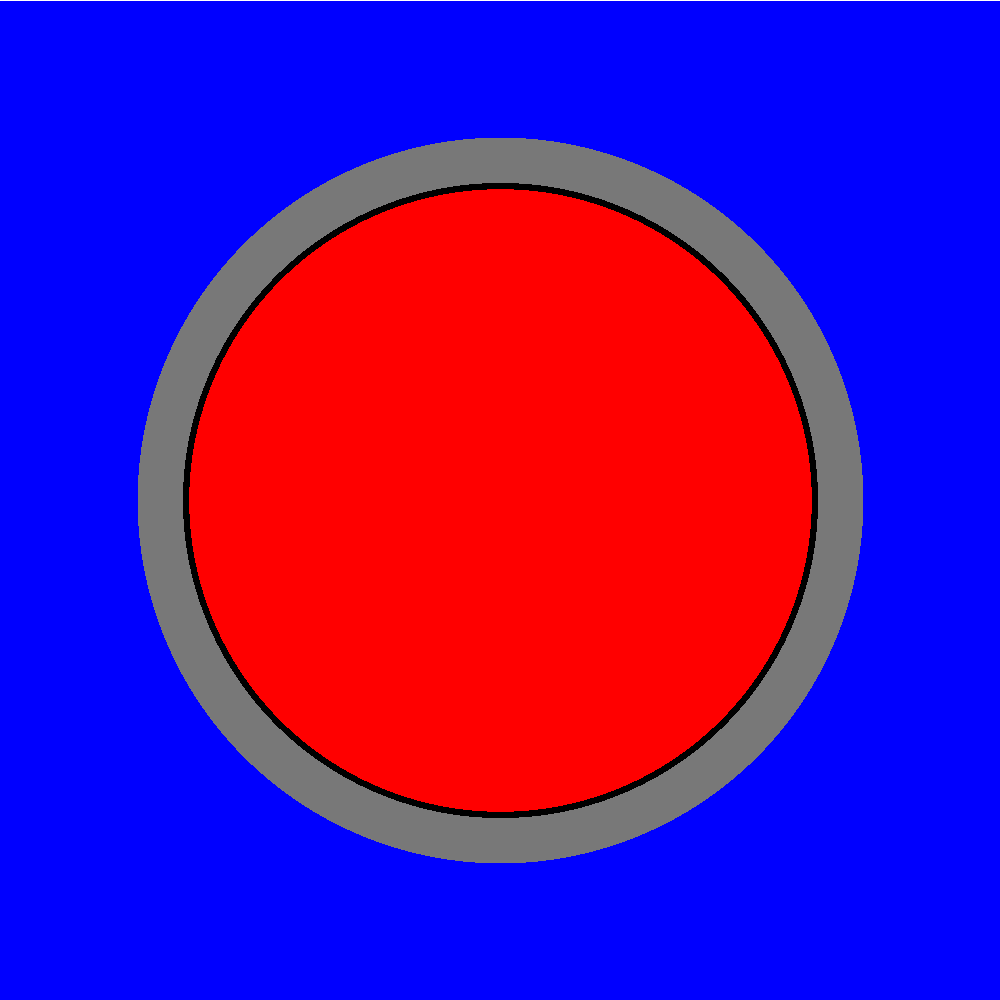
\includegraphics[width=0.9\linewidth]{figures/pin-cell-simple}
  \caption{}
  \label{fig:pin-materials}
\end{subfigure}%
\begin{subfigure}{.25\textwidth}
  \centering
  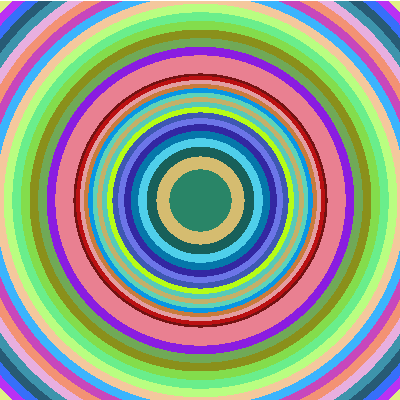
\includegraphics[width=0.9\linewidth]{figures/pin-cell-16x1}
  \caption{}
  \label{fig:pin-rings}
\end{subfigure}
\caption{The PWR fuel pin cell materials (a) and MGXS spatial homogenization zones (b) for the second test case benchmark.}
\label{fig:pin-cell}
\end{figure}

%%%%%%%%%%%%%%%%%%%%%%%%%%%%%%%%%%%%%%%%%%%%%%%%%%%%%%%%%%%%%%%%%%%%%%%%%%%%%%%
\subsection{Simulation Tools}
\label{subsubsec:sim-tools-case2}

The OpenMC continuous energy Monte Carlo code~\citep{romano2013openmc} was employed to generate multi-group cross sections, and reference multi-group reaction rates and fluxes, for the second test case. The \texttt{openmc.mgxs} Python module was used to tally multi-group cross sections in CASMO's seventy energy group structure~\citep{rhodes2006casmo} for each of the radial spatial zones illustrated in Fig.~\ref{fig:pin-rings} from a single eigenvalue calculation. The MGXS were tallied using the scalar flux (Eqn.~\ref{eqn:sigt-mg-scalar}) according to the flux separability approximation. The same Monte Carlo simulation was used to compute a reference eigenvalue, as well as reference multi-group fluxes and reaction rates for each energy group and spatial region. A total of 10 active and 100 inactive batches of 10\textsuperscript{6} particles per batch were simulated. 

The OpenMOC multi-group code~\citep{boyd2014openmoc} was employed to model the second test case benchmark using the MGXS generated by OpenMC. The OpenMOC code is a 2D deterministic method of characteristics code designed for fixed source and eigenvalue neutron transport calculations. The benchmark geometry illustrated in Fig.~\ref{fig:pin-rings} was further discretized for OpenMOC's transport solver with eight azimuthal sectors within each radial ring. A series of multi-group calculations were performed with OpenMOC using the 70-group MGXS tabulated by OpenMC and subsequently collapsed into 1, 2, 8, 16, 25, 40 coarse energy groups. Finally, the OpenMOC eigenvalue and multi-group fluxes were compared with the reference solution computed by OpenMC.

It should be noted that two different OpenMC simulations were performed with different scattering kernels to generate two different MGXS libraries for OpenMOC. The first simulation employed all of the normal scattering physics modeled in OpenMC. The second simulation used OpenMC's ``iso-in-lab'' feature\footnote{The OpenMC ``iso-in-lab'' feature samples the outgoing neutron energy from the scattering laws prescribed by the continuous energy cross section library, but the outgoing neutron direction of motion is sampled from an isotropic in lab distribution.} to enforce isotropic in lab scattering. Although isotropic scattering is not a valid approximation for nuclear reactors, the ``iso-in-lab'' feature enabled comparisons between the reference eigenvalues and reaction rates produced by OpenMC and those computed from isotropic multi-group calculations with OpenMOC. Furthmore, the separate calculations enabled a comparison of the effects due to isotropic in lab scattering and the flux separability approximation.
%%%%%%%%%%%%%%%%%%%%%%%%%%%%%%%%%%%%%%%%%%%%%%%%%%%%%%%%%%%%%%%%%%%%%%%%%%%%%%%
\section{Test Case 1}
\label{sec:test-case1}
%%%%%%%%%%%%%%%%%%%%%%%%%%%%%%%%%%%%%%%%%%%%%%%%%%%%%%%%%%%%%%%%%%%%%%%%%%%%%%%

{\color{red} content to come from Nate's thesis, chapter 9?}

\begin{table}[h!]
  \centering
  \caption{U-238 resonance range reaction rates for collapsed cross sections on simple pin-cell {(\color{red}Table 7.1 from Nate's thesis)}.}
  \label{tab:case1-bias} 
  \begin{tabular}{c c c c c}
  \toprule
  Group & $E_{max}$ [eV] & Reference & Condensed & Error [\%] \\
  \midrule
  15 & 9118.00 & 0.12018 & 0.12030 & 0.102 \\
  16 & 5530.00 & 0.11011 & 0.11027 & 0.142 \\
  17 & 3519.10 & 0.11407 & 0.11444 & 0.330 \\
  18 & 2239.45 & 0.10581 & 0.10630 & 0.457 \\
  19 & 1425.10 & 0.11572 & 0.11625 & 0.461 \\
  20 & 906.899 & 0.21110 & 0.21172 & 0.294 \\
  21 & 367.263 & 0.22169 & 0.22290 & 0.543 \\
  22 & 148.729 & 0.16551 & 0.16649 & 0.598 \\
  23 & 75.5014 & 0.10569 & 0.10621 & 0.487 \\
  24 & 48.0520 & 0.14256 & 0.14394 & 0.964 \\
  25 & 27.7000 & 0.13732 & 0.13867 & 0.984 \\
  26 & 15.9680 & 0.09348 & 0.09348 & 0.001 \\
  27 & 9.87700 & 0.23567 & 0.23813 & 1.041 \\
  \bottomrule
\end{tabular}
\end{table}

\begin{figure}[h!]
  \centering
  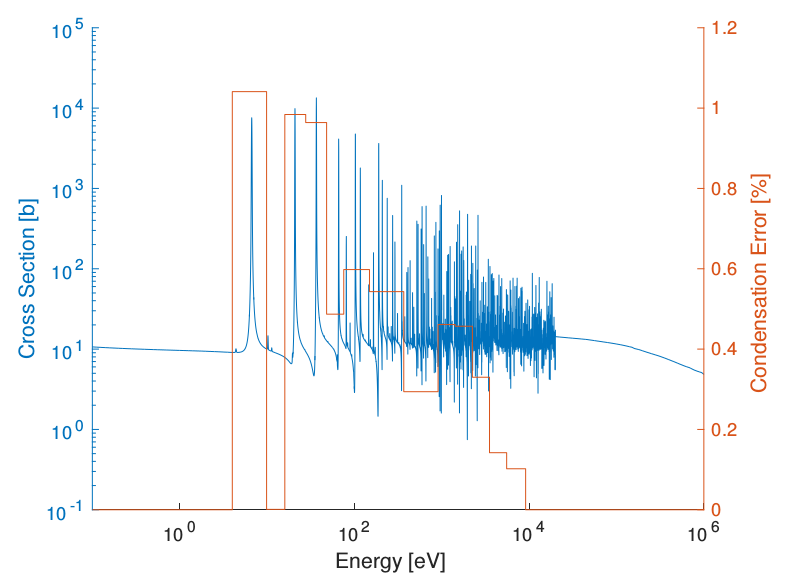
\includegraphics[width=\linewidth]{figures/case1-error}
  \caption{Condensation errors in the resonant groups of the WIMS69 group structure, plotted alongside the U-238 cross section {(\color{red}Figure 7.1 from Nate's thesis)}.}
  \label{fig:case1-errror}
\end{figure}


%%%%%%%%%%%%%%%%%%%%%%%%%%%%%%%%%%%%%%%%%%%%%%%%%%%%%%%%%%%%%%%%%%%%%%%%%%%%%%%
\section{Bias Between Continuous Energy and Multi-Group Calculations}
\label{sec:bias}
%%%%%%%%%%%%%%%%%%%%%%%%%%%%%%%%%%%%%%%%%%%%%%%%%%%%%%%%%%%%%%%%%%%%%%%%%%%%%%%

first paragraph:
-this will come from chapter 5 of my thesis


%%%%%%%%%%%%%%%%%%%%%%%%%%%%%%%%%%%%%%%%%%%%%%%%%%%%%%%%%%%%%%%%%%%%%%%%%%%%%%%
\section{Eigenvalue Bias}
\label{sec:bias-eigenvalues}

first paragraph: what are we comparing??
-reference eigenvalues from MC simulations
-reference MC simulation used to collapse MGXS
-multi-group MOC use MGXS to calculate an eigenvalue
-MG eigenvalue is compared to MC eigenvalue with Eqn.~\ref{eqn:delta-rho}

second paragraph: presented tabulated results
-Tab.~\ref{tab:keff-reference} - reference eigenvalues from OpenMC
  -difference between aniso and iso-in-lab: 65 pcm
-Tab.~\ref{tab:keff-bias-aniso} - OpenMC eigenvalues w/ MGXS generated from anisotropic OpenMC simulations
-Tab.~\ref{tab:keff-bias-iso-in-lab} - OpenMOC eigenvalues w/ MGXS generated from iso-in-lab OpenMC simulations

third paragraph: analyze results
-bias grows more negative with more energy groups
  -goes against intuition: eigenvalues should be more accurate w/ more groups
  -with enough groups (e.g., ultra-fine), MG and MC eigenvalues should match exactly
  -but with coarser group structures, the eigenvalues do not match
    -even with ``perfect'' group condensation with the ``true'' flux

\begin{equation}
\label{eqn:delta-rho}
\Delta\rho = \left(k_{eff}^{OpenMOC} - k_{eff}^{OpenMC}\right) \times 10^{5}
\end{equation}

-data is for 2D fuel pin with MGXS tallied by FSR

\begin{table}[h!]
  \centering
  \caption{Reference OpenMC eigenvalues for a 2D fuel pin.}
  \label{tab:keff-reference} 
  \begin{tabular}{c c}
  \toprule
  {\bf Anisotropic} &
  {\bf Isotropic in Lab} \\
  \midrule
  1.17486 $\pm$ 0.00001 & 1.17421 $\pm$ 0.00001 \\
  \bottomrule
\end{tabular}
\end{table}

\begin{table}[h!]
  \centering
  \caption{The eigenvalue bias with transport-corrected MGXS.}
  \label{tab:keff-bias-aniso} 
  \begin{tabular}{c S[table-format=6.1] S[table-format=6.1] S[table-format=6.1]}
  \toprule
  & \multicolumn{3}{c}{{\bf FSR Discretization}} \\
  \midrule
  \multicolumn{1}{c}{{\bf \# Groups}} &
  {\bf 1$\times$} & {\bf 4$\times$} & {\bf 16$\times$} \\
  \midrule
1 & 53 & 75 & 72 \\
2 & 37 & 1 & 4 \\
4 & -58 & -92 & -109 \\
8 & -74 & -145 & -170 \\
16 & -67 & -154 & -183 \\
25 & -124 & -221 & -245 \\
40 & -130 & -238 & -265 \\
70 & -131 & -281 & -274 \\
  \bottomrule
\end{tabular}
\end{table}

\begin{table}[h!]
  \centering
  \caption{The eigenvalue bias with isotropic-in-lab scattering.}
  \label{tab:keff-bias-iso-in-lab} 
  \begin{tabular}{c S[table-format=6.1] S[table-format=6.1] S[table-format=6.1]}
  \toprule
  & \multicolumn{3}{c}{{\bf FSR Discretization}} \\
  \midrule
  \multicolumn{1}{c}{{\bf \# Groups}} &
  {\bf 1$\times$} & {\bf 4$\times$} & {\bf 16$\times$} \\
  \midrule
1 & 80 & 55 & 66 \\
2 & 141 & 29 & 34 \\
4 & 27 & -43 & -57 \\
8 & 26 & -85 & -102 \\
16 & 35 & -91 & -111 \\
25 & -31 & -158 & -182 \\
40 & -38 & -174 & -202 \\
70 & -39 & -182 & -211 \\
  \bottomrule
\end{tabular}
\end{table}


%%%%%%%%%%%%%%%%%%%%%%%%%%%%%%%%%%%%%%%%%%%%%%%%%%%%%%%%%%%%%%%%%%%%%%%%%%%%%%%
\section{Multi-Group Flux Bias}
\label{sec:bias-flux}

first paragraph: present figures
-Fig.~\ref{fig:rel-err-energy} compares MG and MC flux by energy group
  -innermost and outermost rings of the fuel pin, and average across all rings
-Fig.~\ref{fig:rel-err-space} compares MG and MC flux by spatial zone
  -for three energy group ``ranges'' across all radial rings in the fuel pin
-describe the three energy ranges
  -range A: group for the U-238 capture resonance at 6.67 eV
  -range B: groups spanning the three lowest-lying U-238 capture resonances
  -range C: all U-238 resonance energy groups
  
second paragraph: analyze figures
-take analysis from my thesis
-the errors are largest for range A which most tightly encompasses a single resonance
-errors vary widely across fuel pin
-tie this into an argument of why this:
  (1) causes an eigenvalue bias
  (2) results from loss of angular information with scalar flux-weighted MGXS
-segue into next section on possible solutions

\begin{figure}[h!]
\centering
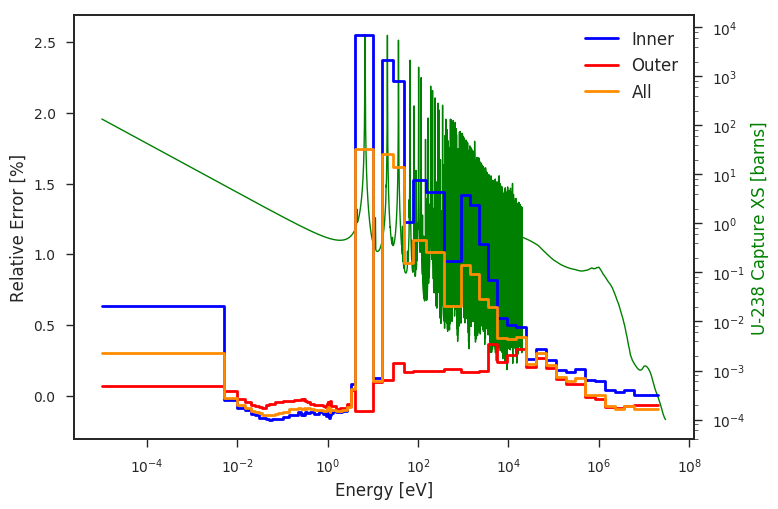
\includegraphics[width=\linewidth]{figures/rel-err-inner-outer}
\caption{The energy-dependent relative error of the OpenMOC scalar flux with respect to the reference OpenMC flux for the innermost, outermost and all FSRs.}
\label{fig:rel-err-energy}
\end{figure}

\begin{figure}[H]
\centering
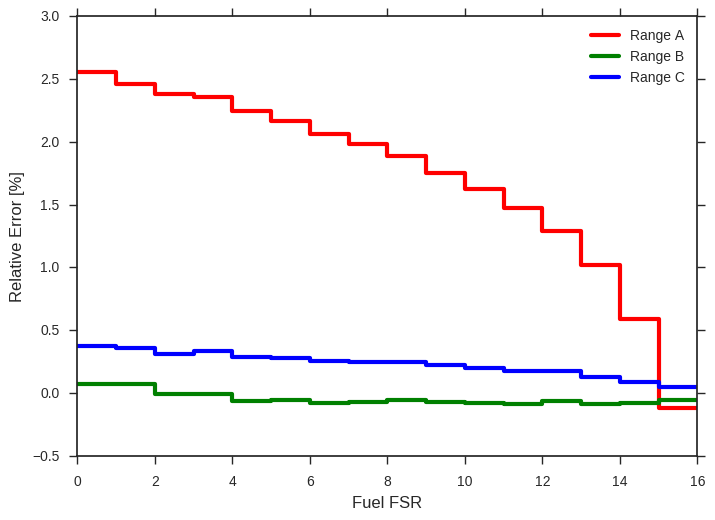
\includegraphics[width=0.8\linewidth]{figures/rel-err-fuel-fsrs}
\caption{The spatially-varying relative error of the OpenMOC scalar flux with respect to the reference OpenMC flux in energy Ranges A, B, and C.}
\label{fig:rel-err-space}
\end{figure}
%%%%%%%%%%%%%%%%%%%%%%%%%%%%%%%%%%%%%%%%%%%%%%%%%%%%%%%%%%%%%%%%%%%%%%%%%%%%%%%
\section{SuPerHomog\'{e}n\'{e}isation Factors}
\label{sec:sph}
%%%%%%%%%%%%%%%%%%%%%%%%%%%%%%%%%%%%%%%%%%%%%%%%%%%%%%%%%%%%%%%%%%%%%%%%%%%%%%%

-angular dependent total MGXS only true solution


%%%%%%%%%%%%%%%%%%%%%%%%%%%%%%%%%%%%%%%%%%%%%%%%%%%%%%%%%%%%%%%%%%%%%%%%%%%%%%%
\subsection{Overview}
\label{subsec:sph-overview}

The SPH algorithm enforces reaction rate preservation between a reference fine-mesh transport problem and a corresponding coarse mesh transport or diffusion problem in energy and space. SPH factors have traditionally been applied to spatially-homogenized few-group MGXS for coarse mesh diffusion applications. However, this section will introduce SPH factors to enforce equivalence between continuous energy Monte Carlo and deterministic multi-group transport methods. 

The SPH scheme postulates the existence of a set of factors $\mu_{k,g}$ for each spatial zone $k$ and energy group $g$ which force the streaming and collision terms in the transport equation to balance with a fixed source $Q_{k,g}$:

\begin{dmath}
\label{eqn:chap6-sph-transport-eqn}
\mathbf{\Omega} \cdot \nabla \psi_{g}(\mathbf{r},\mathbf{\Omega}) + \mu_{k,g}\Sigma_{t,k,g}\psi_{g}(\mathbf{r},\mathbf{\Omega}) = Q_{k,g}(\mathbf{\Omega})
\end{dmath}

\noindent In this equation, the SPH factors are applied to correct the total MGXS in each region and group. The fixed source $Q_{k,g}$ is computed from the reference fine-mesh solution. In this case,  the fixed source is treated as the sum of scattering and fission production sources in each energy group and spatial zone. For example, continuous energy Monte Carlo can be used to compute reference multi-group fluxes and MGXS, which are then combined to compute an isotropic source as follows:

\begin{dmath}
\label{eqn:chap6-sph-source}
Q_{k,g}(\mathbf{\Omega}) = \frac{1}{4\pi} \sum_{g'=1}^{G} \Sigma_{s,k,g' \rightarrow g}\phi_{k,g'} + \frac{\chi_{k,g}}{4\pi k_{eff}}\sum_{g'=1}^{G} \nu\Sigma_{f,k,g'}\phi_{k,g'}
\end{dmath}

\noindent Given the fixed source and total MGXS from MC, Eqn.~\ref{eqn:chap6-sph-transport-eqn} may be solved using any multi-group transport method, such as MOC. The challenge is to devise estimates to the true SPH factors $\mu_{k,g}$ which adequately preserve reaction rates. The following section describes the iterative scheme used to estimate SPH factors.


%%%%%%%%%%%%%%%%%%%%%%%%%%%%%%%%%%%%%%%%%%%%%%%%%%%%%%%%%%%%%%%%%%%%%%%%%%%%%%%
\subsection{Algorithm}
\label{sec:sph-algorithm}

An iterative algorithm is used to estimate SPH factors from a series of multi-group fixed source calculations. First, the estimates $\mu_{k,g}^{(n)}$ at iteration $n$ to the true SPH factors $\mu_{k,g}$ are introduced as a correction factor for the total cross section in Eqn.~\ref{eqn:chap6-sph-transport-eqn}:

\begin{dmath}
\label{eqn:chap6-sph-transport-eqn-iterate}
\mathbf{\Omega} \cdot \nabla \psi_{g}^{(n)}(\mathbf{r},\mathbf{\Omega}) + \mu_{k,g}^{(n-1)}\Sigma_{t,k,g}\psi_{g}^{(n)}(\mathbf{r},\mathbf{\Omega}) = Q_{k,g}(\mathbf{\Omega})
\end{dmath}

\noindent A multi-group transport code (such as OpenMOC) may be used to solve Eqn.~\ref{eqn:chap6-sph-transport-eqn-iterate} with angular and volume integration to compute the scalar flux distribution. The SPH factor estimates $\mu_{k,g}^{(n)}$ are found from the ratio of the reference Monte Carlo scalar flux $\phi_{k,g}^{MC}$ to the flux $\phi_{k,g}^{(n)}$ computed from the fixed source calculation at iteration $n$,

\begin{equation}
\label{eqn:chap6-sph-update}
\mu_{k,g}^{(n)} = \frac{\phi_{k,g}^{MC}}{\phi_{k,g}^{(n)}}
\end{equation}

\noindent where the factors are initialized to unity on the first iteration:

\begin{dmath}
\label{eqn:chap6-sph-initial}
\mu_{k,g}^{(0)} = 1
\end{dmath}

The SPH factors are used to find a total MGXS which forces neutron balance in Eqn.~\ref{eqn:chap6-sph-transport-eqn-iterate}. The initial total MGXS $\Sigma_{t,k,g}^{(0)}$ is computed from the reference MC flux and total reaction rate tallies. The SPH factors are then used to obtain a corrected total MGXS $\Sigma_{t,k,g}^{(n)}$ on each iteration:

\begin{dmath}
\label{eqn:chap6-sph-update-sigt}
\Sigma_{t,k,g}^{(n)} = \mu_{k,g}^{(n-1)}\Sigma_{t,k,g}^{(0)}
\end{dmath}

The series of fixed source problems defined by Eqn.~\ref{eqn:chap6-sph-transport-eqn-iterate} are solved until the SPH factors converge. A common convergence criterion is the maximum relative absolute deviation across energy groups and spatial zones:

\begin{dmath}
\label{eqn:chap6-sph-residual}
res = \max_{k,g} \left|\frac{\mu_{k,g}^{(n)} - \mu_{k,g}^{(n-1)}}{\mu_{k,g}^{(n-1)}}\right|
\end{dmath}

\noindent A residual of 10$^{-7}$ can typically be achieved with twenty or fewer iterations.

The scattering matrix $\Sigma_{s,k,g'\rightarrow g}$ and fission production cross section $\nu\Sigma_{f,k,g}$ are used to compute the reference fixed source in Eqn.~\ref{eqn:chap6-sph-source}, but are not needed in the iterative scheme defined in Eqn.~\ref{eqn:chap6-sph-transport-eqn-iterate}. However, in the context of this thesis, SPH factors are computed to preserve reaction rates in subsequent eigenvalue calculations. Therefore, the SPH factors must be applied to the scattering matrix and fission production cross sections to produce a fully-corrected MGXS library:

\begin{dmath}
\label{eqn:chap6-sph-update-sigs}
\Sigma_{s,k,g'\rightarrow g}^{(n)} = \mu_{k,g}^{(n-1)}\Sigma_{s,k,g'\rightarrow g}^{(0)}
\end{dmath}

\begin{dmath}
\label{eqn:chap6-sph-update-nusigf}
\nu\Sigma_{f,k,g}^{(n)} = \mu_{k,g}^{(n-1)}\nu\Sigma_{f,k,g}^{(0)}
\end{dmath}

It should be noted that although the SPH-corrected MGXS are defined to preserve reaction rates, they will not preserve the group-wise scalar flux. However, the angular or scalar flux may be easily recovered from the fluxes $\tilde{\psi}_{k,g}$ and $\tilde{\phi}_{k,g}$ computed with the SPH-corrected MGXS in an eigenvalue or fixed source calculation:

\begin{dmath}
\label{eqn:chap6-sph-update-angular-flux}
\psi_{k,g} = \mu_{k,g}\tilde{\psi}_{k,g}
\end{dmath}

\begin{dmath}
\label{eqn:chap6-sph-update-scalar-flux}
\phi_{k,g}^{(n)} = \mu_{k,g}\tilde{\phi}_{k,g}
\end{dmath}

The SPH iteration algorithm described here is summarized in Alg.~\ref{alg:chap6-sph}. It should be noted that as presently posed, there is no unique solution to the set of SPH factors which preserve reaction rates. A unique solution may be found by forcing the factors to be unity in non-fissile zones (\textit{e.g.}, moderator, clad and gap)\footnote{A formulation of the SPH algorithm which corrected MGXS in both fissile and non-fissile zones was also implemented. This formulation introduced an outer loop over each spatial zone in Alg.~\ref{alg:chap6-sph}. The scheme is not presented here since it was unstable and the SPH factors diverged after a few outer iterations. Future work may develop a more rigorous approach to preserve reaction rates in each spatial zone.}. This approach is motivated by the fact that resonances which lead to self-shielding errors -- such as the U-238 capture resonances studied in Sec.~\ref{subsec:chap2-angle} -- are generally from isotopes in the fuel. However, the reaction rates in non-fissile zones will not be preserved since the MGXS in these zones remain uncorrected, but these errors are likely dominated by those in the fuel as was shown for the PWR benchmarks in Sec.~\ref{subsec:chap5-diagnosis-rxn-rates}.

\begin{algorithm}[h]
\caption{SPH Factor Algorithm}
\label{alg:chap6-sph}
\begin{algorithmic}[1]
  \State Initialize $\Sigma_{t,k,g}^{(0)}$, $\Sigma_{s,k,g'\rightarrow g}^{(0)}$, $\nu\Sigma_{f,k,g}^{(0)}$, and $\chi_{k,g}^{(0)}$ from MC tallies \Comment{Tab.~\ref{table:chap3-tally-types}}
  \State Compute $Q_{k,g}$ from MC flux and MGXS \Comment{Eqn.~\ref{eqn:chap6-sph-source}}
  \State Initialize $\mu_{k,g}^{(0)}$ to unity
  \While{SPH factor residuals are not converged}
    \State Update $\Sigma_{t,k,g}^{(n)}$ with SPH factors \Comment{Eqn.~\ref{eqn:chap6-sph-update-sigt}}
    \State Solve fixed source transport problem\footnotemark \Comment{Eqn.~\ref{eqn:chap6-sph-transport-eqn-iterate}}
    \State Compute new SPH factors $\mu_{k,g}^{(n)}$ \Comment{Eqn.~\ref{eqn:chap6-sph-update}}
    \State Compute SPH factor residuals \Comment{Eqn.~\ref{eqn:chap6-sph-residual}}
  \EndWhile
  \State Compute final MGXS with SPH factors \Comment{Eqns.~\ref{eqn:chap6-sph-update-sigt},~\ref{eqn:chap6-sph-update-sigs},~\ref{eqn:chap6-sph-update-nusigf}}
\end{algorithmic}
\end{algorithm}

\footnotetext{A series of $G$ independent fixed source problems may be solved for each of the $G$ groups. Alternatively, a single fixed source problem may simultaneously solve for all $G$ groups, as is done in OpenMOC.}


%%%%%%%%%%%%%%%%%%%%%%%%%%%%%%%%%%%%%%%%%%%%%%%%%%%%%%%%%%%%%%%%%%%%%%%%%%%%%%%
\subsection{Results}
\label{sec:sph-results}

-show plot of flux errors with SPH across fuel pin
-results for a 2D fuel pin with MGXS tallied by FSR


\begin{table}[h!]
  \centering
  \caption{The eigenvalue bias with SPH-corrected MGXS.}
  \label{table:keff-bias-sph} 
  \begin{tabular}{c S[table-format=6.1] S[table-format=6.1] S[table-format=6.1]}
  \toprule
  & \multicolumn{3}{c}{{\bf FSR Discretization}} \\
  \midrule
  \multicolumn{1}{c}{{\bf \# Groups}} &
  {\bf 1$\times$} & {\bf 4$\times$} & {\bf 16$\times$} \\
  \midrule
1 & 19 & -18 & -14 \\
2 & 25 & -14 & -6 \\
4 & 7 & 2 & 1 \\
8 & 4 & -0 & 2 \\
16 & 5 & 0 & 4 \\
25 & 5 & 2 & -1 \\
40 & 4 & 3 & -2 \\
70 & 4 & 2 & -3 \\
  \bottomrule
\end{tabular}
\end{table}
%%%%%%%%%%%%%%%%%%%%%%%%%%%%%%%%%%%%%%%%%%%%%%%%%%%%%%%%%%%%%%%%%%%%%%%%%%%%%%%
\section{Conclusions}
\label{sec:conclusions}
%%%%%%%%%%%%%%%%%%%%%%%%%%%%%%%%%%%%%%%%%%%%%%%%%%%%%%%%%%%%%%%%%%%%%%%%%%%%%%%

first paragraph: summary of problem
-recall flux separability approx: use of scalar flux rather than angular flux to weight MGXS
-recall first test case: two-region pin cell with slowing down source
  -used ultra-fine deterministic transport reference solution to collapse MGXS
  -reaction rate errors of over 1\% in groups with largest U-238 capture resonances
-recall second test case: critical four-region PWR pin cell
  -used continous energy MC as reference solution to collapse MGXS with scalar flux-weighted MGXS
  -reaction rate errors led to an eigenvalue bias of approximately 200 pcm due to under-prediction of U-238 capture in resonance groups
-energy and spatial dependence of the bias:
  -the bias emerges / grows with more energy groups
  -reaction rate errors are concentrated in the interior of the fuel pin

second paragraph: solutions
-fully angularly-dependent MGXS
  -demonstrated that it resolves the errors for the two-region pin cell benchmark
-SPH factors
  -equivalence method between continuous energy MC and deterministic transport
  -resolved reaction rate errors and eigenvalue bias for the four-region pin cell benchmark
-angularly-dependent MGXS require memory and are not supported by today's transport codes
-SPH factors suffer from shortcomings

In particular, the SPH scheme requires knowledge of the reference source distribution, is dependent on the spatial discretization mesh, and is indiscriminate between various sources of approximation error.

{\color{red} Future work: jump conditions? coarse angularly-dependent MGXS? universal SPH factors?}

%Although it may be possible to universally apply pre-tabulated SPH factors to fixed geometric configurations, it will likely be necessary to develop alternative methods to account for the angular dependence of the total MGXS. For example, the angular dependence of the total MGXS may be adequately embedded into the scattering kernel using the Consistent-P approximation~\cite{bell1967transport}. Alternatively, a coarse set of angular-dependent MGXS may mitigate most of the bias observed between OpenMC and OpenMOC. For example, a simple approximation might model two different total MGXS for neutrons entering or leaving a fuel pin. Although a coarse angular scheme would not capture the high degree of angular variation illustrated in~\autoref{fig:batman-plots}, it might capture enough to adequately resolve the bias. One challenge to this approach would be to define a general way to accommodate different PWR discretizations within each fuel pin cell.
%%%%%%%%%%%%%%%%%%%%%%%%%%%%%%%%%%%%%%%%%%%%%%%%%%%%%%%%%%%%%%%%%%%%%%%%%%%%%%%
\section*{Acknowledgments}
%%%%%%%%%%%%%%%%%%%%%%%%%%%%%%%%%%%%%%%%%%%%%%%%%%%%%%%%%%%%%%%%%%%%%%%%%%%%%%%


This work was supported by the Idaho National Laboratory and the National Science Foundation Graduate Research Fellowship Grant No. 1122374. This research made use of the resources of the High Performance Computing Center at Idaho National Laboratory, which is supported by the Office of Nuclear Energy of the U.S. Department of Energy and the Nuclear Science User Facilities under Contract No. DE-AC07-05ID14517. The authors' note Adam Nelson's correspondence related to his independent work related to angularly-dependent multi-group cross sections generated with OpenMC.


\section*{References}
\bibliography{references}
\bibliographystyle{annals}

\end{document}
